\documentclass[main.tex]{subfiles}

\begin{document}

\newpage
\section{Progressive Photon Mapping as a Case Study} \label{section:photon}



%%%%%%%%%%%%%%%%%%%%%%%%%%%%
\subsection{The Rendering Equation}

The realistic simulation of illumination of an environment is a complex problem. In theory, a simulation is truly realistic when it completely simulates, or closely approximates, the rendering equation. This equation, first proposed in 1986 \cite{kajiya1986rendering}, is based on the laws of conservation of energy, and describes the total amount of emitted light from any given point, based on incoming light and reflection distribution. The equation is presented in \cref{eq:render}.

\common{equations/rendering}

In short, the equation defines the surface radiance $\surfaceRadiance$, leaving the point $x$ in the direction $\radianceDir$. This is given by $\emittedLight$, which represents light self-emitted by a surface, and $\incidentLight$, which is the radiance along a given incidence direction. $\brdf$ is the \acf{BRDF} and $\Omega$ represents the semi-sphere of incoming directions centered in $x$.


%%%%%%%%%%%%%%%%%%%%%%%%%%%%%
\subsection{Ray Tracing History}

Prior to photon mapping, typical approaches to approximate the rendering equation would use combinations of more than one method, such a Ray Tracing, Radiosity or Metropolis Light Transport \cite{wallace1987two,veach1997metropolis}. Each method attempts to simulate the travel of light particles across the scene, and model the various interactions with the environment, but with different approaches, advantages and limitations.

Ray Tracing methods work by simulating light particles traveling from the eye into the scene, being reflected and refracted until they reach a light source.

Radiosity follows an opposite approach, and simulates the path light takes from the light source, until it reaches the eye. It only deals with diffuse interactions, however, and is commonly used in combination with other techniques.


%%%%%%%%%%%%%%%%%%%%%%%%
\subsection{Photon Mapping}

Photon mapping is based on another method to approximate the rendering equation, first proposed in 1996 \cite{jensen1996global}, and works as two-pass algorithm. In a first pass, photons are traced from the light sources into the scene and stored in a photon map as they interact with the surfaces. This creates a structure that roughly represents the entirety of light within the scene. The second pass is rendering, in which the photon map is used to estimate the illumination in the scene, using common Ray Tracing techniques (for example, Monte Carlo ray tracing). The photon map is used to aid the computation of the total radiance. It is useful not only to increase performance, mostly by allowing a reduction in the number of samples to cast while still providing accurate results, but also to allow the modeling of some light effects that are not preset, or are inefficient to process in other rendering methods.

One case in particular is when light is being transported along a specular to diffuse to specular path (SDS path) illustrated in \cref{fig:sdspath} before reaching the eye. This is what is commonly known as a caustic, such as, for example, the shimmering light seen of the bottom of a pool, or any light source enclosed in glass. This scenario is very common since most artificial light sources are enclosed in glass, but is particularly hard to simulate, particularly when the light source is small, making the sampling probability very low when using Monte Carlo methods.

\begin{figure}[!htp]
  \centering
  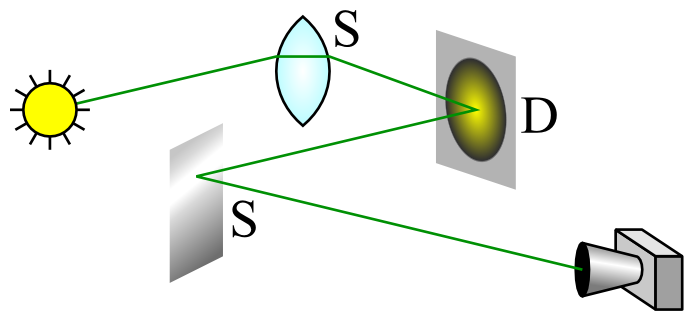
\includegraphics{sds-path}
  \caption{Illustration of a Specular to Diffuse to Specular path (SDS) \label{fig:sdspath}}
\end{figure}

Another example of a typically hard to simulate effect is Subsurface Scattering, which is observed when light enters the surface of a translucent object, is scattered when interacting with the material, and finally exits the surface at a different point. Generally, light will be reflected several times within the surface before backing out an angle different from the one it would have take had it been reflected by the surface. This is visible in materials such as marble, or skin, and can be seen in \cref{fig:subscat}

\begin{figure}[!htp]
  \centering
  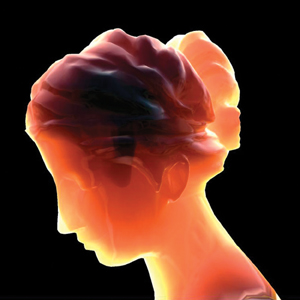
\includegraphics[width=0.3\textwidth]{subsurface-scattering}
  \caption{Subsurface Scattering \label{fig:subscat}}
\end{figure}

Both of these can be simulated well by Photon Mapping algorithms, although a high amount of caustics will hinder performance a lot.


\subsection{Extensions to Photon Mapping}

The algorithm initially proposed \cite{jensen1996global} has been the basis for several improved versions proposed throughout the years.

In 2005, a proposed version introduced the concept of Reverse photon mapping \cite{havran2005fast}, in which the two steps were reversed. The ray tracing step was the first to be computed, and would build an accelerating structure (such as a \textit{kd-tree}), used in the later photon tracing steps to find the nearest hit points that a photon contributes to. This approach would improve performance when large numbers of rays are used.

In 2000, Suykens and Willems \cite{suykens2000adaptive}, and later in Hachisuka, Ogaki and Jensen 2008 \cite{hachisuka2008progressive} attempted an algorithm that would asymptotically converge to a solution, by gradually reducing the search radius of the radiance estimate based on the number of photons already found.

A new formulation of photon Mapping was proposed in 2011 \cite{knaus2011progressive}, which used a probabilistic formulation that allows for a memoryless algorithm, without requiring statistics to be maintained, and removes dependencies between each individual step, allowing them to be calculated independently, and thus being able to run in parallel.

\end{document}
